\input{preambulo_materiales}

\title{Ejercicios de repaso \vspace{-2cm}}
\author{}
\date{ }

%--------------------------------------------------------------------
\newcounter{choice}
\renewcommand\thechoice{\Alph{choice})}
%\newcommand\choicelabel{\thechoice.}
\newcommand\choicelabel{\thechoice}

\newenvironment{choices}%
  {\list{\choicelabel}%
     {\usecounter{choice}\def\makelabel##1{\hss\llap{##1}}%
       \settowidth{\leftmargin}{W.\hskip\labelsep\hskip 2.5em}%
       \def\choice{%
         \item
       } % choice
       \labelwidth\leftmargin\advance\labelwidth-\labelsep
       \topsep=0pt
       \partopsep=0pt
     }%
  }%
  {\endlist}

\newenvironment{oneparchoices}%
  {%
    \setcounter{choice}{0}%
    \def\choice{%
      \refstepcounter{choice}%
      \ifnum\value{choice}>1\relax
        \penalty -50\hskip 1em plus 1em\relax
      \fi
      \choicelabel
      \nobreak\enskip
    }% choice
    % If we're continuing the paragraph containing the question,
    % then leave a bit of space before the first choice:
    \ifvmode\else\enskip\fi
    \ignorespaces
  }%
  {}
%----------------------------------------------------------

\begin{document}
\maketitle
\fontsize{14}{14}\selectfont

Resuelve los siguientes ejercicios:

\begin{enumerate}
\item Jaime cargó la bolsa del mandado cuando acompañó a su mamá. La mamá compró $2$ kilogramos y medio de naranjas, tres cuartos de kilogramo de limones, una papaya de 2 kilogramos y $250$ gramos, un kilogramo y medio de tomates y $250$ gramos de chiles. ¿Cuánto cargó Jaime en total? \hspace{0.3cm} \textbf{R.} \rule{3cm}{0.1mm}
\item ¿Qué fracción de una hora son $12$ minutos? ¿Cuál es el número decimal correspondiente? \hspace{0.3cm} \textbf{R.} \rule{3cm}{0.1mm}
\item Óscar tiene dos amigas estadounidenses. Britney gastó $\dfrac{4}{5}$ de dólar en comprar un chocolate y Jenny gastó $75$ centavos de dólar en comprar otro. ¿A quién le costó más el chocolate? \hspace{0.3cm} \textbf{R.} \rule{3cm}{0.1mm}
\item En la siguiente recta númerica, localiza los puntos $\dfrac{1}{5}$, $\dfrac{11}{10}$, $0.9$, $1.5$ y $\dfrac{7}{5}$. Luego escribe estos números en orden de menor a mayor.
\begin{figure}[H]
    \centering
    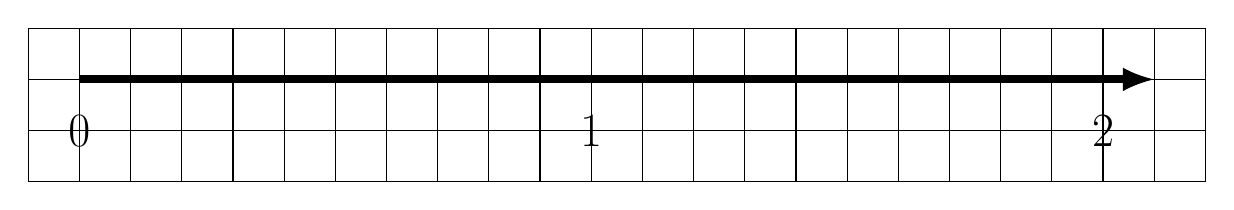
\begin{tikzpicture}[scale=0.65]
        \draw[thin] (0, 0) grid (23, 3) rectangle (0, 0);
        \draw[-latex,line width=1mm] (1, 2) -- (22, 2);
        \node at (1, 1) {\LARGE $0$};
        \node at (11, 1) {\LARGE $1$};
        \node at (21, 1) {\LARGE $2$};
    \end{tikzpicture}
\end{figure}
\vspace{0.5cm}
\item Ayer, Martín caminó $\dfrac{1}{4}$ de kilómetro durante los primeros $10$ minutos, $400$ metros durante los siguientes $10$ minutos y $\dfrac{4}{5}$ de kilómetro durante los terceros $10$ minutos. ¿Cuántos kilómetros caminó durante esa media hora? \hspace{0.3cm} \textbf{R.} \rule{3cm}{0.1mm}
\item Calcula la medida de los ángulos $a, b, c, d, e$ de los siguientes triángulos:
\begin{figure}[H]
  \centering
  \includegraphics[scale=0.65]{Imagenes/Angulos_01.png}
\end{figure} 
\item Traza una recta numérica en la cuadrícula y localiza las fracciones $\dfrac{2}{3}$, $\dfrac{5}{4}$ y $\dfrac{11}{6}$
\begin{figure}[H]
    \centering
    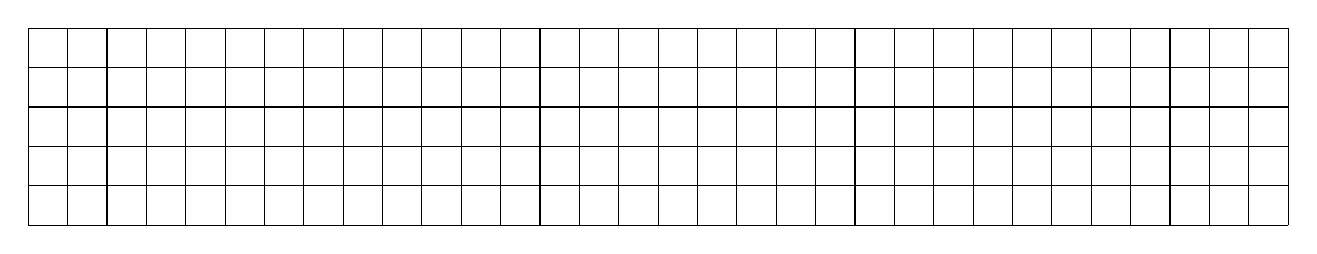
\begin{tikzpicture}
        \draw[step=0.5, thin] (0, 0) grid (16, 2.5);
    \end{tikzpicture}
\end{figure}
\item En la siguiente recta numérica están localizados los números $-2, 5, 4, 2,$ \\
$5$ y $-6$.
\begin{figure}[H]
  \centering
  \begin{tikzpicture}
    \draw (-7.3, 0) -- (7.3, 0);
    \foreach \x in {-7, -6,..., 6, 7}
      \draw (\x, -0.2) -- (\x, 0.2);
    
    \node at (0, -0.5) {$0$};
    \node at (-6, 0.5) {F};
    \node at (-5, 0.5) {E};
    \node at (-2, 0.5) {D};
    \node at (2, 0.5) {C};
    \node at (4, 0.5) {B};
    \node at (5, 0.5) {A};
  \end{tikzpicture}
\end{figure}

\begin{enumerate}[label=\alph*)]
\item Escribe el número que corresponda a cada letra:
\\
A = \rule{1cm}{0.1mm} \hspace{0.2cm} B = \rule{1cm}{0.1mm} \hspace{0.2cm} C = \rule{1cm}{0.1mm} \hspace{0.2cm} D = \rule{1cm}{0.1mm} \hspace{0.2cm} \\ E = \rule{1cm}{0.1mm} \hspace{0.2cm} F = \rule{1cm}{0.1mm} \hspace{0.2cm}
\item ¿Cuál de los números está más lejos del cero? A = \rule{1cm}{0.1mm}
\item ¿Cuál está más cerca del cero? A = \rule{1cm}{0.1mm}
\item ¿Alguna pareja de números está a la misma distancia del cero (no importa si está a la derecha o la izquierda)? \rule{1cm}{0.1mm} \hspace{0.2cm} En caso afirmativo, ¿cuáles son esos números? A = \rule{2cm}{0.1mm} 
\end{enumerate}
\item Una empresa vende autopartes a varias distribuidoras y registra semanalmente cuánto le pagó cada una por los artículos que le envió.
\begin{table}[H]
  \centering
  \large
  \begin{tabular}{| c | l |} \hline
    Distribuidora & Monto en pesos \\ \hline
    A & $12500$ \\ \hline
    B & $-8700$ \\ \hline
    C & $5450$ \\ \hline
    D & $-10200$ \\ \hline
    E & $-5500$ \\ \hline
  \end{tabular}
\end{table}
\begin{enumerate}[label=\alph*)]
\item ¿¿Cuáles distribuidoras le deben dinero a la empresa? \textbf{R.} \rule{2cm}{0.1mm}
\item ¿Cuál de ellas le debe más dinero? \textbf{R.} \rule{2cm}{0.1mm}
\item ¿Cuál le debe menos? \textbf{R.} \rule{2cm}{0.1mm}
\item ¿Cuáles distribuidoras le pagaron a la empresa? \textbf{R.} \rule{2cm}{0.1mm}
\item ¿Cuáles de las distribuidoras le pagó menos? \textbf{R.} \rule{2cm}{0.1mm}
\item ¿Cuánto dinero en total recibió la empresa? \textbf{R.} \rule{2cm}{0.1mm}
\item ¿Cuánto dinero en total le deben a la empresa? \textbf{R.} \rule{2cm}{0.1mm}
\end{enumerate}
\item Realiza las siguiente sumas de números con signo:
\begin{enumerate}[label=\alph*)]
\item $9 + (-5) = $ \textbf{R.} \rule{2cm}{0.1mm}
\item $(-3) + 2 = $ \textbf{R.} \rule{2cm}{0.1mm}
\item $3.51 + (-3.45) = $ \textbf{R.} \rule{2cm}{0.1mm}
\item $(-11.6) + (-9.18) = $ \textbf{R.} \rule{2cm}{0.1mm}
\item $\left(- \dfrac{5}{8} \right) + \left(- \dfrac{3}{4} \right) + \left( \dfrac{1}{2} \right) = $ \textbf{R.} \rule{2cm}{0.1mm}
\end{enumerate}
\end{enumerate}

\end{document}